%-------------------------------------------------------------------------------
% yum_effects
%-------------------------------------------------------------------------------
%
% \file        yum_effects.tex
% \library     Documents
% \author      Chris Ahlstrom
% \date        2015-06-05
% \update      2018-05-26
% \version     $Revision$
% \license     $XPC_GPL_LICENSE$
%
%     Provides the effectsxx section of yoshimi-user-manual.tex.
%
%-------------------------------------------------------------------------------

\section{Effects}
\label{sec:effects}

   The \textsl{Yoshimi} \textbf{Effects} panel provides a number of special
   effects that can be applied to parts.
   Effects are, generally, blackboxes that transform audio signals in a
   specified way. More exactly, the only input data for an effect in
   \textsl{Yoshimi} is an array of samples.
   The output is the transformed array of samples.

   As described, effects have no information about anything else. For
   example, key presses are not recognized. Therefore, pressing a key does
   not initiate the LFO. Phase knobs will always be relative to a global LFO,
   dependent only on the system time.

   \textsl{Wetness} determines the mix of the results of the effect and its
   input.  This mix is made at the effects output. If an effect is wet, it
   means that nothing of the input signal is bypassing the effect. If it is
   dry, then the effect has no effect.

   \textsl{Interpolation}
   means that, if one MIDI-learns the controls, one can now automate them
   smoothly instead of the somewhat gritty previous behaviour.
   This does not change processor demand when running at 64 frames, a short
   number of frames.
   This interpolation is especially effective on "saw" sounds with the
   frequency control on the EQ low pass filter.


   The \textbf{Effects} panel is shown in
   \figureref{fig:yoshimi_main_screen}.
   Note that these effects have been incorporated into a separate
   guitar-effects project called \textsl{Rakkarrak} \cite{rakarrack}.

   There are two types of effects: System effects and Insertion effects.
   Insertion effects have a sub-type for part effects. The effects themselves
   behave in the same way but with slightly different 'outer' controls.

   The System effects apply to all parts and allows one to set the amount of
   effect that applies to each part. Also, it is possible to send the output
   of one system effect to another system effect. In the user interface this
   is shown as "source -\textless destination". For example:
   The \textbf{0 -\textless 1} knob controls how
   much of the system effect 0 is sent to system effect 1.

   Insertion effects are described in
   \sectionref{subsubsec:effects_paneltypes_insertion}.

\subsection{Effects / Panel Types}
\label{subsec:effects_paneltypes}

   There are three variations of Effects sub-panels:

   \begin{itemize}
      \item \textbf{System Effects}.
      \item \textbf{Insertion Effects}.
      \item \textbf{Part/Instrument Effects}.
   \end{itemize}

   Here are the major elements of the main effects panel, which shows the
   System and Insertion effects tabs.

\begin{figure}[H]
   \centering
   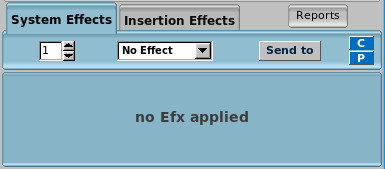
\includegraphics[scale=0.75]{effects-panel/system-effects.jpg}
   \caption{System Effects Dialog}
   \label{fig:system_effects_dialog}
\end{figure}

   \begin{enumber}
      \item \textbf{System Effects Tab}
      \item \textbf{Effect Number}
      \item \textbf{Effect Name}
      \item \textbf{Send to}
      \item \textbf{C}
      \item \textbf{P}
      \item \textbf{Effects Panel}
      \item \textbf{Insertion Effects Tab}
      \item \textbf{Reports}
   \end{enumber}

   \setcounter{ItemCounter}{0}      % Reset the ItemCounter for this list.

   \itempar{System Effects Tab}{effects!system tab}
   System Effects Tab.
   The items in this tab are described in the next few paragraphs.

   \itempar{Effect Number}{effects!number}
   Effect Number.
   Up to 8 effects can be supported at one time by one part.

   \itempar{Effect Name}{effects!name}
   Effect Name.

   Values: \texttt{No Effect*, Reverb, Echo, Chorus, Phaser, AlienWah,
      Distortion, EQ, DynFilter}

\begin{figure}[H]
   \centering
   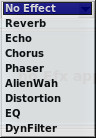
\includegraphics[scale=1.0]{effects-panel/system-effects-selections.jpg}
   \caption{Effects Names}
   \label{fig:effects_names}
\end{figure}

   \itempar{Send to}{effects!send to}
   Effects Send To.
   Each knob controls how much of the system effect indicated by the left
   number is sent to the system effect indicated by the right number.
   This user-interface drop-down is shown only in the
   \textbf{Part / Edit / Effects} version of the effects panel.

   Values: \texttt{Next Effect, Part Out, Dry Out}

\begin{figure}[H]
   \centering
   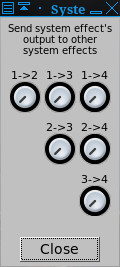
\includegraphics[scale=1.0]{effects-panel/system-effects-send-to.jpg}
   \caption{Effects, Send To}
   \label{fig:effects_send_to}
\end{figure}

   \itempar{C}{effects!copy dialog}
   Copy-to-clipboard Dialog.
   We need to learn more about how this dialog gets populated.

\begin{figure}[H]
   \centering
   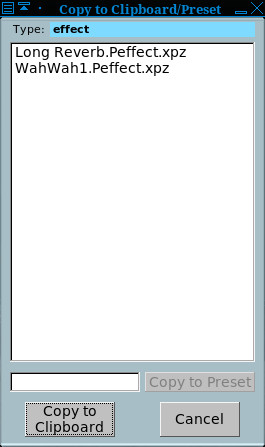
\includegraphics[scale=0.75]{effects-panel/system-effects-C-clipboard.jpg}
   \caption{Effects / Copy To Clipboard}
   \label{fig:effects_copy_to_clipboard}
\end{figure}

   Note that, in recent versions of \textsl{Yoshimi}, the Type label at the top
   is not "effect", but "Peffect".  What does this mean?

   \itempar{P}{effects!paste dialog}
   Paste-from-clipboard Dialog.
   We need to learn more about how this dialog gets populated.

\begin{figure}[H]
   \centering
   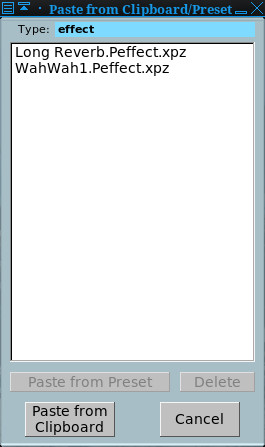
\includegraphics[scale=0.75]{effects-panel/system-effects-P-clipboard.jpg}
   \caption{Effects / Paste From Clipboard}
   \label{fig:effects_paste_from_clipboard}
\end{figure}

   \itempar{Effects Panel}{effects!panel}
   Effects Panel.
   This area is filled by the controls for the selected effect.

   \itempar{Insertion Effects Tab}{effects!insertion tab}
   Insertion Effects Tab.
   The items in this tab are described below,
   in the \ref{subsubsec:effects_paneltypes_insertion}
   sub-section.

   \itempar{Reports}{effects!reports}
   Effects Reports.

\begin{figure}[H]
   \centering
   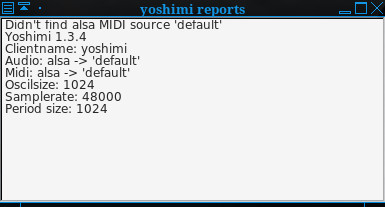
\includegraphics[scale=1.0]{effects-panel/reports.jpg}
   \caption{Effects / Reports}
   \label{fig:effects_reports}
\end{figure}

   The next sub-sections show the variations on the effects panels, using the
   DynFilter effect as the subject effects panel.

\subsubsection{Effects / Panel Types / System }
\label{subsubsec:effects_paneltypes_system}

   The first variation
   appears when you enable an effect in the
   \textbf{System Effects}
   panel of the main \textsl{Yoshimi} dialog.  It contains the standard
   controls for the given effect, plus the following interface items.

\begin{figure}[H]
   \centering
   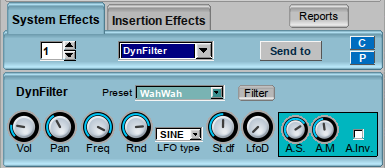
\includegraphics[scale=1.0]{bottom-panel/instrument-edit/Effects/system-effects-panel.png}
   \caption{Sample System Effects Dialog}
   \label{fig:sample_system_effects_dialog}
\end{figure}

   \begin{enumber}
      \item \textbf{Effect number}
      \item \textbf{Effect selection}
      \item \textbf{Effect Filter}
      \item \textbf{C}
      \item \textbf{P}
   \end{enumber}

\subsubsection{Effects / Panel Types / Insertion }
\label{subsubsec:effects_paneltypes_insertion}

   The second effects variation
   appears when you enable an effect in the
   \textbf{Insertion Effects}
   panel of the main \textsl{Yoshimi} dialog.
   It contains the standard
   controls for the given effect, plus the following interface items.

\begin{figure}[H]
   \centering
   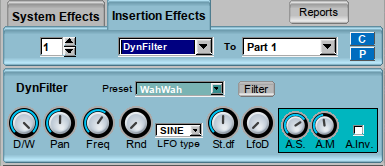
\includegraphics[scale=1.0]{bottom-panel/instrument-edit/Effects/insertion-effects-panel.png}
   \caption{Sample Insertions Effects Dialog}
   \label{fig:sample_insertion_effects_dialog}
\end{figure}

   \begin{enumber}
      \item \textbf{Effect number}
      \item \textbf{Effect selection}
      \item \textbf{To}
      \item \textbf{C}
      \item \textbf{P}
   \end{enumber}

   The insertion effects apply to one part or to the master output.
   One may use more
   than one insertion effect for one part or the master output.
   If using more than one effect, the
   effects with smaller indexes will be applied first (first, insertion
   effect 0 occurs, then effect 1, and so on).
   If the part selected for insertion
   effect is \texttt{-1} then the effect will be \textsl{disabled};
   \index{insertion effect!-1}
   \index{insertion effect!disable}
   if the part is \texttt{-2} the
   effect will be applied to Master Out.
   \index{insertion effect!-2}
   \index{insertion effect!master out}

   \setcounter{ItemCounter}{0}      % Reset the ItemCounter for this list.

   \itempar{To}{effects!to}
   Send the Effect To.

\begin{figure}[H]
   \centering
   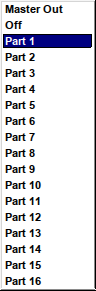
\includegraphics[scale=1.0]{bottom-panel/instrument-edit/Effects/part-selection-dropdown.png}
   \caption{Part Selection Dropdown}
   \label{fig:sample_part_selection_dropdown}
\end{figure}

\subsubsection{Effects / Panel Types / Instrument }
\label{subsubsec:effects_paneltypes_instrument}

   There is also a "part" or "instrument" effects window which is accessed
   by going to the main window, clicking the \textbf{Edit} button in the
   bottom panel to open the edit dialog, and then clicking the
   \textbf{Effects} button there.  The part effects window has the
   same layout as System and Insertion effects; it is now almost identical
   to Insertion effects.

   It contains the standard controls for the given effect, plus the
   following interface items.

   \begin{enumber}
      \item \textbf{Effect number}
      \item \textbf{Effect selection}
      \item \textbf{To} (part-selection-dropdown.png)
      \item \textbf{C}
      \item \textbf{P}
      \item \textbf{Bypass}
      \item \textbf{Close}
   \end{enumber}

   "To" Values: \texttt{Master Out, Off, Part 1, Part 2, ..., Part 16}

\begin{figure}[H]
   \centering
   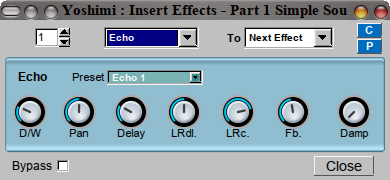
\includegraphics[scale=1.0]{1.3.9/effects-edit-echo.png}
   \caption{Sample Instrument Effects Dialog}
   \label{fig:sample_instrument_effects_dialog}
\end{figure}

   \index{effects!bypass}
   Note the extra \textbf{Bypass} check-box.  If the \textbf{Bypass} item is
   checked, then the effect is not used; it is taken out of the circuit.  This
   user-interface item only appears if one clicks the \textbf{Edit} button for
   a Part, and then clicks the \textbf{Effects} button in the \textbf{Edit}
   window.

   Also be aware that the layout of some of the effects dialogs have been modified
   in the latest revisions of \textsl{Yoshimi}.
   This dialog form is reversed (top and bottom) with the latest
   \textsl{Yoshimi}, and slightly simplified in appearance. This was done to more
   closely match the layout of the System and Insertion Effects.
   Also, in the actual effects, some control positions and sizes have been changed
   to improve readbility.

\subsection{Effects / Upgrade}
\label{subsec:effects_upgrade}
   Since V 1.5.11 there is an indication that effect controls have been altered. As can
   be seen, the normal pale cyan background of the preset selector becomes a strong blue.
   This colour change will also apply to any effects that have been saved.
   \begin{figure}[H]
   \centering
   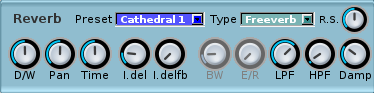
\includegraphics[scale=1.0]{1.5.11/effects_warning.png}
%   \caption{Effects Edit, No Effect}
   \label{fig:effects_warning}
\end{figure}

   This change will take place if you alter any of the controls after a preset has been
   selected. The rationale here is that one can make such changes, then save the
   Instrument/Patchset that this effect is in.
   When re-loading, one would be quite likely to forget that changes have been made and
   experimentally switch to different presets or even different effects.
   Previously, at this point those changes have been lost and one might be puzzed that
   the sound has changed (possibly quite subtly) when returning to the same preset.

   With the new upgrade one is warned about this. It even applies when loading very old
   Instruments and Patchsets as the effects are checked against the known defaults as
   they are installed.

\subsection{Effects / None}
\label{subsec:effects_edit_none}

\begin{figure}[H]
   \centering
   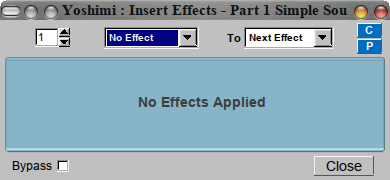
\includegraphics[scale=1.0]{1.3.9/effects-edit-none.png}
   \caption{Effects Edit, No Effect}
   \label{fig:effects_edit_none}
\end{figure}

\subsection{Effects / DynFilter}
\label{subsec:effects_edit_dynfilter}

   A dynamic filter is, as the name says, a filter which changes its
   parameters dynamically, dependent on the input and current time. In
   \textsl{ZynAddSubFX}, frequency is the only variable parameter. It can be
   used as an "envelope following filter" (sometimes referenced "Auto Wah" or
   simply "envelope filter").

\subsubsection{Effects / DynFilter / Circuit}
\label{subsubsec:effects_edit_dynfilter_circuit}

   Though this filter might look a bit complicated, it is actually easy. We
   divide the parameters into two classes:

   \begin{itemize}
      \item Filter Parameters are the ones obtained when one clicks on Filter.
         They give the filter its basic settings.
      \item Effect Parameters are the other ones that control how the filter
         changes.
   \end{itemize}

   The filter basically works like this: The input signal is passed through a
   filter which dynamically changes its frequency. The frequency is an
   additive of:

   \begin{itemize}
      \item The filter’s base frequency.
      \item An LFO from the effect parameters.
      \item The "amplitude" of the input wave.
   \end{itemize}

   The amplitude of the input wave is not the current amplitude, but the so
   called "Root Mean Square (RMS)" value. This means that we build a mean on
   the current amplitude and the past values. How much the new amplitude
   takes influence is determined by the Amplitude Smoothness (see below).

   RMS value plays an important role in the term \textsl{loudness}.
   A fully distorted signal can sound 20 db louder due to its higher RMS value.
   This filter takes this into account, depending on the smoothness.

\begin{figure}[H]
   \centering
   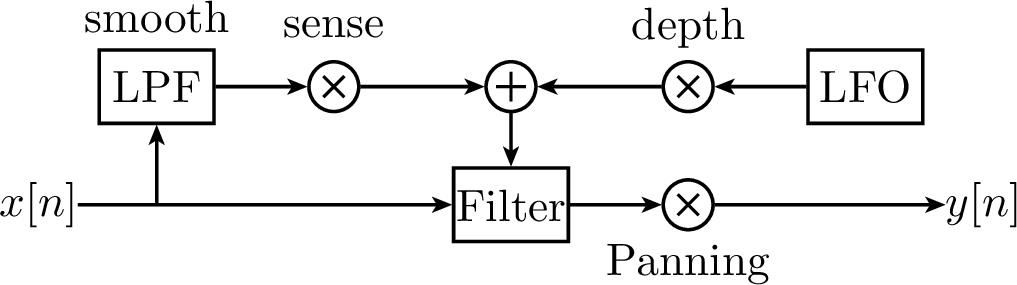
\includegraphics[scale=0.25]{zyn/effects/dynamic.png}
   \caption{Dynamic Filter Circuit Diagram}
   \label{fig:dynfilter_circuit_diagram}
\end{figure}

\subsubsection{Effects / DynFilter / User Interface}
\label{subsubsec:effects_edit_dynfilter_ui}

\begin{figure}[H]
   \centering
%  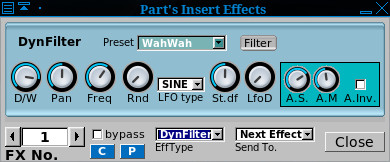
\includegraphics[scale=1.0]{bottom-panel/instrument-edit/Effects/effects-edit-dynfilter.jpg}
   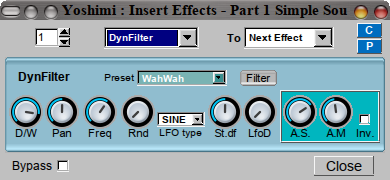
\includegraphics[scale=1.0]{1.3.9/effects-edit-dynfilter.png}
   \caption{Effects Edit, DynFilter}
   \label{fig:effects_edit_dynfilter}
\end{figure}

   This figure shows the Part/Instrument variation of the DynFilter sub-panel.
   The System/Insertion variation has the following elements.

   \begin{enumber}
      \item \textbf{Preset}
      \item \textbf{Filter}
      \item \textbf{Vol} (system/insertion) or \textbf{D/W} (part/instrument)
      \item \textbf{Pan}
      \item \textbf{Freq}
      \item \textbf{Rnd}
      \item \textbf{LFO Type}
      \item \textbf{St.df}
      \item \textbf{LfoD}
      \item \textbf{A.S.}
      \item \textbf{A.M.}
      \item \textbf{Inv.}
   \end{enumber}

   This figure shows an additional section, in the bottom panel of the effect's
   user-interface.
   See \sectionref{subsubsec:effects_edit_reverb_ui}, which
   describes these elements in more detail.
   However, it seems that all but the \textbf{bypass} control and
   the \textbf{Close} button have been removed
   from the latest versions of \textsl{Yoshimi}.

   \begin{enumber}
      \item \textbf{FX No.} (an unlabelled number "wheel")
      \item \textbf{bypass} (bottom panel)
      \item \textbf{EffType} (now unlabelled, obvious from context)
      \item \textbf{To} (where the effect is sent to)
      \item \textbf{C}
      \item \textbf{P}
      \item \textbf{Close} (bottom panel)
   \end{enumber}

   The four controls in the middle of the middle panel
   (\textbf{Freq}, \textbf{Rnd}, \textbf{LFO Type}, and \textbf{St.df})
   control the LFO.

   In \textbf{DynFilter}, the \textbf{Gain} control, and most of the formant
   filter ones only operate as one \textsl{releases} the mouse button, and the
   scroll wheel cannot be used at all.  Investigating, it was found that this
   was specifically done because these controls create significant noise when
   adjusted, and effects are real time, so that's a lot of noise. (When filters
   are applied elsewhere, the result is next-note so one doesn't hear the
   changes).

   Which is more desirable:
   (1) Noise when ever the control is moved, scroll wheel capability and fully
   responsive GUI;
   (2) Noise only when the control is released, no scroll wheel, filter graphs
   only updated on control release.
   To be determined.

   Let's start with the user-interface elements present in the
   System/Insertion variation of this effect.

   \setcounter{ItemCounter}{0}      % Reset the ItemCounter for this list.

   \itempar{Preset}{dynfilter!preset}
   DynFilter Preset.

\begin{figure}[H]
   \centering
   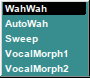
\includegraphics[scale=1.0]{bottom-panel/instrument-edit/Effects/dynfilter-presets.png}
   \caption{DynFilter Presets}
   \label{fig:effects_dynfilter_presets}
\end{figure}

   Values: \texttt{WahWah, AutoWah, Sweep, VocalMorph1, VocalMorph2}

   \itempar{Filter}{dynfilter!filter}
   DynFilter Filter.

   This small button brings up Filter Params stock sub-panel item.
   This stock user-interface item is shown and described in
   \sectionref{subsubsec:filter_parameters_user_interface}.

   \itempar{Vol}{dynfilter!volume}
   DynFilter Volume.

   Values: \textsl{0 to 127}

   If the effect is used as a System effect, then this control appears.

   \itempar{D/W}{dynfilter!dry/wet}
   DynFilter Dry/Wet Mix Setting.

   Values: \textsl{0 to 127}

   If the effect is used as an Insertion effect, then this control appears.
   "Dry" means the unprocessed signal and "wet" means the processed signal.

   \itempar{Pan}{dynfilter!pan}
   DynFilter Panning.

   Values: \textsl{0 to 127}

   After the input signal has passed through the filter, Pan can apply
   panning.

   \itempar{Freq}{dynfilter!lfo freq}
   DynFilter LFO Frequency.

   Values: \textsl{0 to 127}

   \itempar{Rnd}{dynfilter!lfo randomness}
   DynFilter LFO Randomness.

   Values: \textsl{0 to 127}

   \itempar{LFO Type}{dynfilter!lfo type}
   DynFilter LFO Type.

   \itempar{St.df}{dynfilter!lfo stdf}
   DynFilter LFO.
   Left/right channel phase shift.

   \itempar{LfoD}{dynfilter!lfo depth}
   DynFilter LFO Depth.
   This control is one that helps define the mix of the LFO and the
   amplitude.

   \itempar{A.S}{dynfilter!a.s.}
   DynFilter A.S.
   This control is one that helps define the mix of the LFO and the
   amplitude.
   A.S sets the Amplitude Sensing (i.e. how much influence the amplitude
   shall have).

   \itempar{A.M}{dynfilter!a.m.}
   DynFilter A.M.
   One of two knobs let one control the way how the RMS value of the
   amplitudes is measured.
   A.M sets the Amplitude Smoothness (this is described above). The higher
   one sets this value, the more slowly will the filter react.

   \itempar{Inv.}{dynfilter!a.inv}
   DynFilter A.Inv.  One of two knobs let one control the way how the RMS
   value of the amplitudes is measured.  A.Inv., if set, negates the
   (absolute) RMS value. This will lower the filter frequency instead of
   increasing it. Note that this will not have much effect if the effects
   input is not very loud.

\subsubsection{Effects / DynFilter / NRPN Values}
\label{subsubsec:effects_edit_dynfilter_nrpn}

   Effects can be controlled via "non-registered parameter numbers", or NRPNs.
   This section will eventually (we hope)
   detail the NRPN values supported by the DynFilter effect.

   For more information on the concept of NRPNs, see
   \sectionref{subsubsec:concepts_midi_nrpn}.

% ----------------------------------------------------------

\subsection{Effects / AlienWah}
\label{subsec:effects_edit_alienwah}

   AlienWah is a nice effect done by Paul Nasca. It resembles a vocal morpher
   or wahwah a bit, but it is more strange. That's why he called it "AlienWah"
   The effect is a feedback delay with complex numbers.

   The AlienWah effect is a special, dynamic formant filter.
   Paul Nasca named it AlienWah because it sounded "a bit like
   wahwah, but more strange". The result of the filter is a sound varying
   between the vocals "Ahhhhh" (or "Uhhhhh") and "Eeeeee".

\subsubsection{Effects / AlienWah / Circuit}
\label{subsubsec:effects_edit_alienwah_circuit}

   No diagram, just a description of AlienWah.

   Hint: Keep in mind that Effects that can be controlled by LFO can also be
   controlled arbitrarily: Set the LFO depth to zero and manipulate the phase
   knob (e.g. with NRPNs or maybe via OSC in the future).

   The way that the filter moves between the two vocals is mainly described
   by an LFO. A bit easified, Paul Nasca has stated the formula (for
   i2 = -1 and R \textless 1) as

   \[fb=R*(cos(a)+i*sin(a))\]

   \[yn=yn-delay*R*(cos(a)+i*sin(a))+xn*(1-R).\]

   The input xn has the real part of the samples from the wavefile and the
   imaginary part is zero. The output of this effect is the real part of
   \texttt{yn}.
   \texttt{a} is the phase.

\subsubsection{Effects / AlienWah / User Interface}
\label{subsubsec:effects_edit_alienwah_ui}

\begin{figure}[H]
   \centering
%  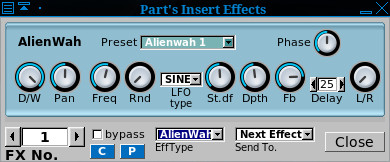
\includegraphics[scale=1.0]{bottom-panel/instrument-edit/Effects/effects-edit-alienwah.jpg}
   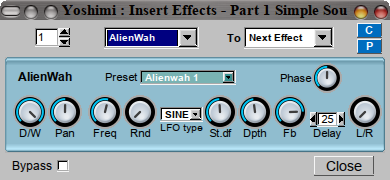
\includegraphics[scale=1.0]{1.3.9/effects-edit-alienwah.png}
   \caption{Effects Edit, AlienWah}
   \label{fig:effects_edit_alienwah}
\end{figure}

   \begin{enumber}
      \item \textbf{Preset}
      \item \textbf{Phase}
      \item \textbf{Vol} or \textbf{D/W}
      \item \textbf{Pan}
      \item \textbf{Freq}
      \item \textbf{Rnd}
      \item \textbf{LFO type}
      \item \textbf{St.df.}
      \item \textbf{Dpth}
      \item \textbf{Fb.}
      \item \textbf{Delay}
      \item \textbf{L/R}
   \end{enumber}

   \setcounter{ItemCounter}{0}      % Reset the ItemCounter for this list.

   \itempar{Preset}{alienwah!preset}
   AlienWah Preset.

   Values: \texttt{AlienWah 1, AlienWah 2, AlienWah 3, AlienWah 4}

   \itempar{Phase}{alienwah!phase}
   The phase of the AlienWah.
   See \texttt{a} in the above formula.
   This lets one set where the vocal is between
   "Ahhhhh" and "Eeeeee".

   \itempar{Vol}{alienwah!volume}
   AlienWah Volume.

   Values: \texttt{0 to 127}

   The volume control is present is this effect is used as an insertion
   effect.

   \itempar{D/W}{alienwah!dry/wet}
   AlienWah Dry/Wet.

   Values: \texttt{0 to 127}

   The \textbf{Vol} control is replaced by this control if the effect is
   used as an Insertion effect.

   \itempar{Freq}{alienwah!lfo frequency}
   LFO Frequency.

   Values: \texttt{0 to 127}

   Determines the LFO’s frequency in relative units.

   \itempar{Rnd}{alienwah!lfo randomness}
   LFO Amplitude Randomness.

   Values: \texttt{0 to 127}

   Part of the LFO definition.

   \itempar{LFO type}{alienwah!lfo shape}
   Set the LFO shape.

   Values: \texttt{SINE, TRI}

   Part of the LFO definition.
   Note that the LFO in other contexts has ramps and exponential shapes that
   are not present here.

   \itempar{St.df}{alienwah!phase diff}
   AlienWah Left/Right Chanell Phase Difference.

   Values: \texttt{0 to 127}

   Part of the LFO definition.
   Sets the phase difference between LFO for left/right channels.
   \textbf{St.df} lets one determine how much left and right LFO are phase
   shifted.  64.0 means stereo, higher values increase the right LFO
   relatively to the left one.

   \itempar{Dpth}{alienwah!depth}
   LFO depth.

   Values: \texttt{0 to 127}

   \textbf{Dpth} is a multiplier to the LFO. Thus, it determines
   the LFO's amplitude and its influence.

   \itempar{Delay}{alienwah!delay}
   Amount of delay before the feedback.

   Values: \texttt{1 to 100}

   If this value is low, the sound is turned more into a "wah-wah"-effect.

   \itempar{Fb}{alienwah!feedback}
   AlienWah Feedback.

   Values: \texttt{0 to 127}

   \index{todo!alienwah feedback}
   TODO: What is the effect of the AlienWah feedback setting?

   \itempar{L/R}{alienwah!l/r}
   Determines how the left/right channels are routed to output:

   \begin{itemize}
      \item \textsl{Leftmost/0}. Left to left and right to right.
      \item \textsl{Middle/64}. Left+right to mono.
      \item \textsl{Rightmost/127}. Left to right, and right to left.
   \end{itemize}

   L/R applies crossover at the end of every stage. This is currently not
   implemented for the Analog Phaser.

   \itempar{Subtract}{alienwah!subtract}
   The output is inversed (inverted?)

\subsubsection{Effects / AlienWah / NRPN Values}
\label{subsubsec:effects_edit_alienwah_nrpn}

Effects can be controlled via "non-registered parameter numbers", or NRPNs.
This section details the value supported by the AlienWah effect.

\subsection{Effects / Chorus}
\label{subsec:effects_edit_chorus}

   In a chorus, many people sing together. Even if each of them sings at
   exactly the same frequency, all their voices usually sound different. We
   say they have a different timbre. Timbre is the way we perceive sound and
   makes us differ between different music instruments. This is, physically,
   achieved by varying both the amplitude envelope and the frequency
   spectrum. Multiple sounds with slightly different timbres make a sound
   more shimmering, or powerful. This is called the chorus effect.

   The chorus effect can be achieved by multiple people singing together. In
   a concert, there are many instruments, resulting in the same effect. When
   making electronic music, we only have an input wave and need to generate
   these different timbres by ourselves. ZynAddSubFX therefore simply plays
   the sound, pitch modulated by an LFO, and adds this to the original sound.
   This explains the diagram below: The multiple pitches are generated by a
   delayed version of the input. This version is being pitched by an LFO.
   More detailed, this pitch is generated by varying the reading speed of
   the delayed sound; the variation amount is controlled by an LFO.

   Related effects to Chorus are Flangers. Flangers can be described as
   Chorus with very short LFO delay and little LFO depth. One can imagine a
   flanger as two copies of a sound playing at almost the same time. This
   leads to interference, which can be clearly heared. It is popular to apply
   flangers to guitars, giving them more "character".

\subsubsection{Effects / Chorus / Circuit}
\label{subsubsec:effects_edit_chorus_circuit}

\begin{figure}[H]
   \centering
   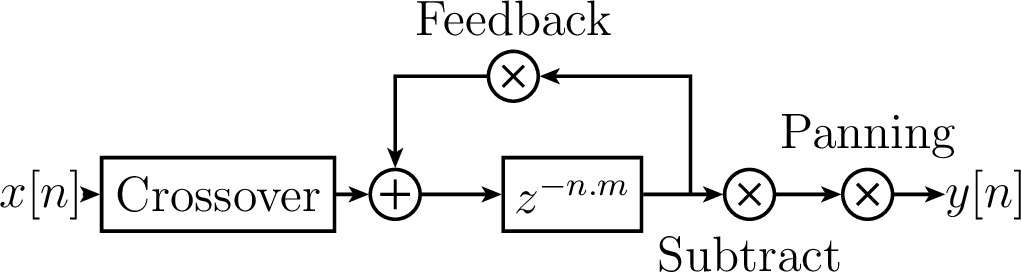
\includegraphics[scale=0.25]{zyn/effects/chorus.png}
   \caption{Chorus Circuit Diagram}
   \label{fig:chorus_circuit_diagram}
\end{figure}

   First, crossover is applied.
   The \textbf{Freq}, \textbf{Rnd}, \textbf{LFO Type}, \textbf{St.df},
   \textbf{Depth} knobs control the LFO
   for the pitch. If the depth is set to zero, the pitch will not be changed
   at all.

   Delay is the time that the delayed sound is delayed "on average". Note
   that the delay also depends on the current pitch.

   After the correct element of the sound buffer is found using the LFO, the
   Fb knob lets one set how loud it shall be played. This is mostly redundant
   to the D/W knob, but we have not applied panning and substraction yet.

   Next, the signal can be negated. If the \textbf{Subtract}
   checkbox is activated, the amplitude is multiplied by -1.

   Finally, \textbf{Pan} lets one apply panning.

\subsubsection{Effects / Chorus / User Interface}
\label{subsubsec:effects_edit_chorus_ui}

\begin{figure}[H]
   \centering
%  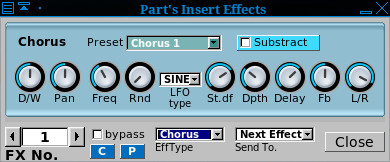
\includegraphics[scale=1.0]{bottom-panel/instrument-edit/Effects/effects-edit-chorus.jpg}
   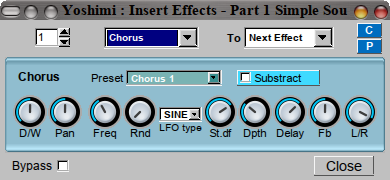
\includegraphics[scale=1.0]{1.3.9/effects-edit-chorus.png}
   \caption{Effects Edit, Chorus}
   \label{fig:effects_edit_chorus}
\end{figure}

   \begin{enumber}
      \item \textbf{Freq}
      \item \textbf{Rnd}
      \item \textbf{LFO type}
      \item \textbf{St.df.}
      \item \textbf{Dpth}
      \item \textbf{Delay}
      \item \textbf{Fb.}
      \item \textbf{L/R}
      \item \textbf{Subtract}
   \end{enumber}

   \setcounter{ItemCounter}{0}      % Reset the ItemCounter for this list.

   \itempar{Freq}{chorus!lfo freq}
   Chorus LFO Frequency.

   \itempar{Rnd}{chorus!lfo randomness}
   Chorus LFO randomness.

   \itempar{LFO type}{chorus!lfo type}
   Set the LFO shape.

   \itempar{St.df}{chorus!l/r phase}
   The phase difference between LFO for left/right channels .

   \itempar{Dpth}{chorus!lfo depth}
   Chorus LFO depth.

   \itempar{Delay}{chorus!delay}
   Delay of the chorus.
   If one uses low delays and LFO depths, this will result in a flanger
   effect.

   \itempar{Fb}{chorus!feedback}
   Chorus Feedback.

   \itempar{L/R}{chorus!l/r routing}
   How the left/right channels are routed to output:

      \begin{enumber}
         \item leftmost. Left to left and right to right.
         \item middle. Left+right to mono.
         \item rightmost. Left to right, and right to left.
      \end{enumber}

   \itempar{Subtract}{chorus!substract}
   The Chorus output is inversed (inverted?)

\subsubsection{Effects / Chorus / NRPN Values}
\label{subsubsec:effects_edit_chorus_nrpn}

Effects can be controlled via "non-registered parameter numbers", or NRPNs.
This section details the value supported by the Chorus effect.

\subsection{Effects / Distortion}
\label{subsec:effects_edit_distortion}

   Distortion means, in general, altering a signal. Natural instruments
   usually produce sine-like waves. A wave is transformed in an unnatural way
   when distortion is used. The most distorted waves are usually pulse waves.
   It is typical for distortion to add overtones to a sound. Distortion often
   increases the power and the loudness of a signal, while the dB level is
   not increased. This is an important topic in the Loudness War.

   As distortion increases loudness, distorted music can cause ear damage at
   lower volume levels. Thus, one might want to use it carefully.
   Distortion can happen in many situations when working with audio. Often,
   this is not wanted. In classical music, for example, distortion does not
   occur naturally. However, distortion can also be a wanted effect. It is
   typical for Rock guitars, but also present in electronic music, mostly in
   Dubstep and DrumNBass.

   The basic components of distortion are mainly

   \begin{itemize}
      \item A preamplifier.
      \item The waveshaping function.
      \item Filters.
   \end{itemize}

   Preamplification changes the volume before the wave is shaped, and is
   indeed the amount of distortion. For example, if one clips a signal, the
   louder the input gets, the more distortion one will get. This can have
   different meanings for different types of distortions, as described below.

   The filters are practical. A reason for using them afterwards is that
   distortion can lead to waves with undesired high frequency parts. Those
   can be filtered out using the LPF. A reason for using filters before
   applying is to achieve multiband distortion. ZynAddSubFX has no "real"
   multiband distortion by now, however.

   The topic of types of distortion is discussed in the
   Oscillator Section.

   Note that one can use the Oscillator editor in order
   to find out what the distortion effect does. Also note that while the
   Oscillator editor’s distortion is limited to some oscillators one can
   produce in the Oscillator editor, the distortion effect can be used on
   every wave that one can generate with \textsl{ZynAddSubFX}.

\subsubsection{Effects / Distortion / Circuit}
\label{subsubsec:effects_edit_distortion_circuit}

   We explain the functionality in a diagram and list the components below.

\begin{figure}[H]
   \centering
   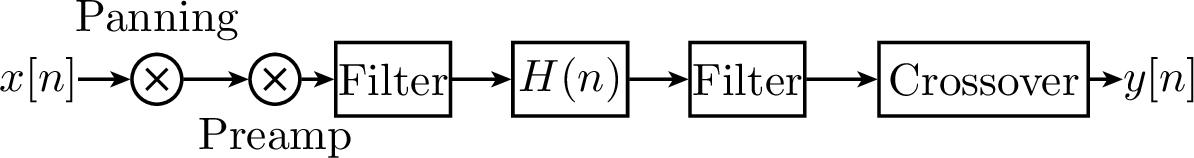
\includegraphics[scale=0.333]{zyn/effects/distort.png}
   \caption{Distortion Circuit Diagram}
   \label{fig:distortion_circuit_diagram}
\end{figure}

   Negation is the first thing to happen. If the \textbf{Neg Checkbox} is
   activated, the amplitude is multiplied by -1.

   \index{distortion effect!panning}
   Panning is applied. Note, however, that one must activate the Stereo
   Checkbox, labelled \textbf{St}, before it will work.

   Pre-amplification is done next. The amount can be changed using the Drive
   nob. Indeed, this is the amount of distortion. For example, if one clips a
   signal, the louder the input gets, the more distortion one will get. This
   can have different meanings for different types of distortion, as
   described above.

   HPF and LPF are filters with 2 poles. Whether they are used before or
   after the waveshape, depends on the checkbox labeled PF.

   The next step is the wave shape. This defines how the wave is actually
   modified. The Type ComboBox lets one define how. We will discuss some
   types below.

   After the wave shape, we scale the level again. This is called output
   amplification. One can change the value using the Level knob.

   Crossover is the last step. This is controlled by the knob LR Mix and
   means that afterwards, a percentage of the left side is applied to the
   right side, and, synchronously, the other way round. It is a kind of
   interpolation between left and right. If one sets the LR Mix to 0.0, one
   will always have a stereo output.

\subsubsection{Effects / Distortion / User Interface}
\label{subsubsec:effects_edit_distortion_ui}

\begin{figure}[H]
   \centering
%  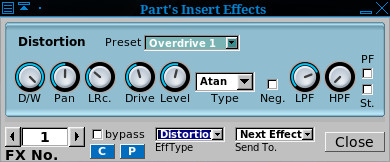
\includegraphics[scale=1.0]{bottom-panel/instrument-edit/Effects/effects-edit-distortion.jpg}
   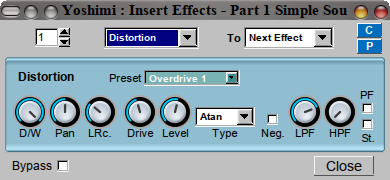
\includegraphics[scale=1.0]{1.3.9/effects-edit-distortion.png}
   \caption{Effects Edit, Distortion}
   \label{fig:effects_edit_distortion}
\end{figure}

   \begin{enumber}
      \item \textbf{Drive}
      \item \textbf{Level}
      \item \textbf{Type}
      \item \textbf{Neg.}
      \item \textbf{LPF}
      \item \textbf{HPF}
      \item \textbf{St.}
   \end{enumber}

   \setcounter{ItemCounter}{0}      % Reset the ItemCounter for this list.

   \itempar{Drive}{distortion!drive}
   Set the amount of distortion.

   \itempar{Level}{distortion!level}
   Amplify or reduce the signal after distortion.

   \itempar{Type}{distortion!type}
   Set the function of the distortion (like arctangent, sine).

   \itempar{Neg}{distortion!negate}
   Negates the amplitude (invert the signal).

   \itempar{LPF}{distortion!lpf}
   Low Pass Filter.

   \itempar{HPF}{distortion!hpf}
   High Pass Filter.

   \itempar{St}{distortion!stereo}
   Set the distortion mode (stereo or mono, checked is stereo).

\subsubsection{Effects / Distortion / NRPN Values}
\label{subsubsec:effects_edit_distortion_nrpn}

   Effects can be controlled via "non-registered parameter numbers", or NRPNs.
   This section details the value supported by the Distortion effect.

\subsection{Effects / Echo}
\label{subsec:effects_edit_echo}

   The echo effect, also known as delay effect, simulates the natural
   reflection of a sound. The listener can hear the sound multiple times,
   usually decreasing in volume. Echos can be useful to fill empty parts of
   songs with.

\subsubsection{Effects / Echo / Circuit}
\label{subsubsec:effects_edit_echo_circuit}

   The good circuit diagram is shown in an old printout we have, but the
   current version of the Echo description at
   http://zynaddsubfx.sourceforge.net/Doc/ shows a
   junk file.  So Paul Nasca's description will have to suffice.

% \begin{figure}[H]
%    \centering
%    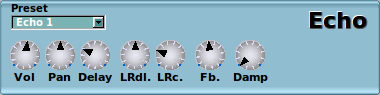
\includegraphics[scale=0.25]{zyn/effects/echo.png}
%    \caption{Echo Circuit Diagram}
%    \label{fig:echo_circuit_diagram}
% \end{figure}

   In ZynAddSubFX, the echo is basically implemented as the addition of the
   current sound and a delayed version of it. The delay is implemented as in
   the picture below. First, we add the delayed signal to the effect input.
   Then, they pass an LP1. This shall simulate the effect of dampening, which
   means that low and especially high frequencies get lost earlier over
   distance than middle frequencies do. Next, the sound is delayed, and then
   it will be output and added to the input.

   The exact formula in the source code for the dampening effect is as
   follows:

   \[Y(t)=(1-d)*X(t)+d*Y(t-1)\]

   where t be the time index for the input buffer, d be the dampening amount
   and X,Y be the input, respective the output of the dampening. This solves
   to

   \[Y(z)=Z(Y(t))=(1-d)*X(z)+d*Y(z)*z-1 <==> H(z)=Y(z)X(z)=1-d1-d*z-1\]

   which is used in \(Y(z)=H(z)*X(z)\). So H(z) is indeed a filter, and by
   looking at it, we see that it is an LP1. Note that infinite looping for
   d=1 is impossible.

\subsubsection{Effects / Echo / User Interface}
\label{subsubsec:effects_edit_echo_ui}

\begin{figure}[H]
   \centering
%  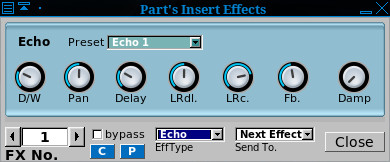
\includegraphics[scale=1.0]{bottom-panel/instrument-edit/Effects/effects-edit-echo.jpg}
   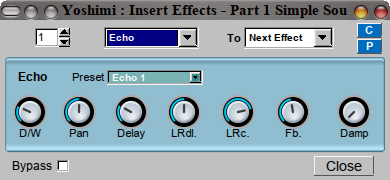
\includegraphics[scale=1.0]{1.3.9/effects-edit-echo.png}
   \caption{Effects Edit, Echo}
   \label{fig:effects_edit_echo}
\end{figure}

   TODO (yoshimi):  Pan lets one apply panning of the input.

   \begin{enumber}
      \item \textbf{Delay}
      \item \textbf{LRdl.}
      \item \textbf{LRc.}
      \item \textbf{Fb.}
      \item \textbf{Damp}
   \end{enumber}

   \setcounter{ItemCounter}{0}      % Reset the ItemCounter for this list.

   \itempar {Delay}{echo!delay}
   The delay time of one echo.

   \itempar {LRdl}{echo!l/r delay}
   Left-Right-Delay.
   The delay between left/right channels.
   If it is set to the middle, then both sides are delayed equally. If
   not, then the left echo comes earlier and the right echo comes (the
   same amount) later than the average echo; or the other way round.
   Set the knob to 0 to hear on the right first.

   \itempar {LRc}{echo!crossover}
   Echo Crossover.
   The "crossing" between left/right channels.

   \itempar {Fb}{echo!feedback}
   Echo feedback.
   Feedback describes how much of the delay is added back to the input.
   Set Fb. to the maximum to hear an infinite echo, or to the minimum to
   just hear a single repeat.

   \itempar {Damp}{echo!damp}
   Echo damping.
   How high frequencies are damped in the Echo effect.
   The Damp value lets the LP1 reject higher frequencies earlier if
   increased.

\subsubsection{Effects / Echo / NRPN Values}
\label{subsubsec:effects_edit_echo_nrpn}

   Effects can be controlled via "non-registered parameter numbers", or NRPNs.
   This section details the value supported by the Echo effect.  TODO.

\subsection{Effects / EQ}
\label{subsec:effects_edit_eq}

   EQ is a parametric equalizer.
   An equalizer is a filter effect that applies different volume to different
   frequencies of the input signal. This can, for example, be used to "filter
   out" unwanted frequencies. ZynAddSubFX’s implementations follow the
   "Cookbook formulae for audio EQ" (\cite{cookbookeq})
   by Robert Bristow-Johnson.

   On the equalizer graph there are 3 white
   vertical bars for 100Hz, 1kHz, 10kHz.

\subsubsection{Effects / EQ / Circuit}
\label{subsubsec:effects_edit_eq_circuit}

% No such figure:
%
% \begin{figure}[H]
%    \centering
%    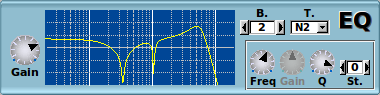
\includegraphics[scale=0.25]{zyn/effects/eq.png}
%    \caption{EQ Circuit Diagram}
%    \label{fig:eq_circuit_diagram}
% \end{figure}

\subsubsection{Effects / EQ / User Interface}
\label{subsubsec:effects_edit_eq_ui}

\begin{figure}[H]
   \centering
%  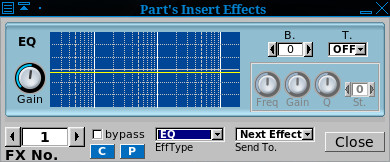
\includegraphics[scale=1.0]{bottom-panel/instrument-edit/Effects/effects-edit-eq.jpg}
   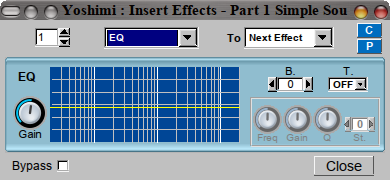
\includegraphics[scale=1.0]{1.3.9/effects-edit-EQ.png}
   \caption{Effects Edit, EQ}
   \label{fig:effects_edit_eq}
\end{figure}

   We describe all parts of the GUI here. The term passband (or often just
   "band") refers to the amount of frequencies which are not
   significantly attenuated by the filter.

   \begin{enumber}
      \item \textbf{Gain}
      \item \textbf{Graph}
      \item \textbf{B}
      \item \textbf{T}
      \item \textbf{Freq}
      \item \textbf{Gain}
      \item \textbf{Q}
      \item \textbf{St}
   \end{enumber}

   Global:

   \setcounter{ItemCounter}{0}      % Reset the ItemCounter for this list.

   \itempar{Gain}{eq!gain}
   Amplifies or reduce the signal that passes through EQ.

   \itempar{Graph}{eq!graph}
   Shows the graph of the EQ frequency response, based on the
   two \textbf{Gain} settings,
   \textbf{T.},
   \textbf{Gain},
   \textbf{Gain},

   \itempar{B}{eq!band}
   Set the current frequency band number (or filter).
   B lets one choose the passband number. Multiple passbands define one
   filter. This is important if one wants multiple filters to be called
   after each other. Note that filters are commutative.

   Values: \texttt{0*, 1, ... 7}

   Bands:

   \itempar{T}{eq!filter type}
   Set the type of the filter.

   Values: \texttt{Off*, Lp1, Hp1, Lp2, Hp2, Bp2, N2, Pk, Lsh, Hsh}

   Note that, for certain values of the \textbf{B} parameter, some of the
   \textbf{T} values will not be available.

   \itempar{Freq}{eq!filter freq}
   The frequency of the filter.
   Freq describes the frequencies where the filter has its poles. For some
   filters, this is called the "cutoff" frequency. Note, however, that a
   bandpass filter has two cutoff frequencies.

   \itempar{Gain (Filter)}{eq!filter gain}
   The gain of the filter.
   Gain is only active for some filters
   (\textbf{Pk}, \textbf{Lsh}, and \textbf{Hsh},
   and it sets the amount of a special
   peak these filters have. Note that for those filters, using the
   predefined gain makes them effectless.

   \itempar{Q}{eq!filter q}
   The Q (resonance, or bandwidth) of the filter.
   Resonance lets one describe a peak at the given frequency for filters
   with 2 poles. This can be compared to real physical objects that have
   more gain at their resonance frequency.

   \itempar{St}{eq!stages}
   Number of additional times the filter will be applied (in
   order to do very steep roll-off - eg. 48 dB/octave).
   St. lets one define multiple filter stages. This is equivalent to
   having multiple copies of the same filter in sequence.

   Values: \texttt{0*, 1, ... 4}

\subsubsection{Effects / EQ / NRPN Values}
\label{subsubsec:effects_edit_eq_nrpn}

   Effects can be controlled via "non-registered parameter numbers", or NRPNs.
   This section details the value supported by the EQ effect.

   TODO.

\subsection{Effects / Phaser}
\label{subsec:effects_edit_phaser}

   The Phaser is a special dynamic filter. The result is a sweeping sound,
   which is often used on instruments with a large frequency band, like
   guitars or strings. This makes it typical for genres like rock or funk,
   where it is often modulated with a pedal, but also for giving strings a
   warm, relaxing character.

\subsubsection{Effects / Phaser / Circuit}
\label{subsubsec:effects_edit_phaser_circuit}

   We explain the functionality in a diagram and list the components below.

\begin{figure}[H]
   \centering
   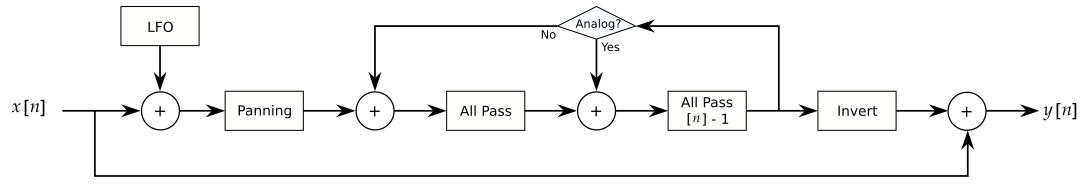
\includegraphics[scale=0.6]{1.5.11/effects-drawing-phaser.png}
   \caption{Phaser Circuit}
   \label{fig:phaser_circuit}
\end{figure}

   The audio signal is split into two paths. One path remains unchanged. The
   other one is sent to a delay line. The delay time (the so-called phase) is
   made dependent on the frequency. Therefore, an all-pass filter is applied
   to the signal, which preserves the amplitude, but determines the delay
   time. At the end, both paths are added.

   Yoshimi offers different types of phasers:

   \begin{itemize}
      \item \textbf{Analog and "normal" phasers}.
      Analog phasers are more complicated.
      They sound punchier, while normal phasers sound more fluently. However,
      analog filters usually need more filter stages to reach a
      characteristic sound.
      \item \textbf{Sine and triangle filters}.
      Note that an analog triangle filter
      with many poles is a barber pole filter and can be used to generate
      Shepard Tones, i.e. tones that seem to increase or decrease with time,
      but do not really.
      \item \textbf{The LFO function can be squared}.
      This is only available for the Analog phaser and converts the triangle
      wave into a hyper sine wave this approximates a triangle for the top
      half, and more rounded sine-like bottom half. The sine squared is simply
      a faster sine wave.
   \end{itemize}

%  TODO: Barber is deactivated, since PLFOtype is only 0 or 1?

   For the normal phaser,
   \figureref{fig:effects_edit_phaser}, below, shows the controls referred to
   in this list of steps.

   \begin{enumber}
      \item First, the LFO is generated.
         There are 4 controls
         (\textbf{Freq}, \textbf{Rnd}, \textbf{LFO} type, \textbf{St.df})
         that define the LFO.
      \item \textbf{Phase} and \textbf{Depth} are added in the usual way.
      \item If \textbf{hyper} is set, then the LFO function is squared.
      \item Next, this modulates the input signal amplitude.
      \item The \textbf{Analog} setting decides whether the phaser is analog
            or "normal".
            For the analog phaser (see the \textbf{Analog} check-box),
            \textbf{L/R} is not implemented.
            Converely, for the normal phaser, \textbf{hyper} and \textbf{dist}
            are not available.
      \item \textbf{Pan} applies panning to the original input in every loop.
      \item Next, phasing is applied - barber-pole type for \textbf{Analog} only.
      \item Then, based on the setting of \textbf{Stages}, further phasing
            stages are applied.
            For \textbf{Analog} only the \textbf{dist} control sets the amount of
            distortion when applying the phasing stages.
      \item \textbf{Fb} applies feedback next. The last sound buffer element is (after
            phasing) multiplied by this value and then added back in. For the
            normal filter, the value is added before, and, for analog, after the
            first phasing stage.
      \item Finally, the \textbf{Sub.} option inverts the signal, multiplying it
            by -1.
   \end{enumber}

\subsubsection{Effects / Phaser / User Interface}
\label{subsubsec:effects_edit_phaser_ui}

\begin{figure}[H]
   \centering
   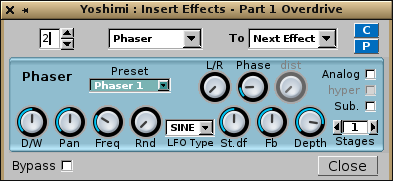
\includegraphics[scale=1.0]{1.5.11/effects-edit-phaser.png}
   \caption{Effects Edit, Phaser}
   \label{fig:effects_edit_phaser}
\end{figure}

%  TODO. Include the item-paragraphs for each GUI element.

   \begin{enumber}
      \item \textbf{Preset.}
      \item \textbf{Depth}
      \item \textbf{Phase}
      \item \textbf{Stages}
      \item \textbf{Sub.}
      \item \textbf{hyper}
      \item \textbf{Analog}
      \item \textbf{D/W}
      \item \textbf{Pan}
      \item \textbf{Freq}
      \item \textbf{Rnd}
      \item \textbf{St.df}
      \item \textbf{Fb}
      \item \textbf{L/R}
      \item \textbf{dist}
      \item \textbf{LFO}
   \end{enumber}

   The extra fields that are shown if the effect is an insertion effect are
   not shown.  They are still need to be described.

   \itempar{Preset}{phaser!preset}
   Phaser Presets.

%  TODO: need a diagram of the dropdown

   Values: \texttt{Phaser 1, ...}

%  TODO.

   \itempar{Depth}{phaser!depth}
   Phaser Depth. Phaser LFO Depth?

   Values: \texttt{0\% to 100\%}

   \itempar{Phase}{phaser!phase}
   Phaser Phase.

   Values: \texttt{0\% to 100\%}

   \itempar{Stages}{phaser!stages}
   Phaser Stages.

   Values: \texttt{1*, 2, ... 12}

   \itempar{Sub.}{phaser!Subtract}
   Phaser Subtract.
   Checking this box inverts the output.

   Values: \texttt{Off*, On}

   \itempar{hyper}{phaser!hyper}
   Phaser Hyper.
   Checking this box sets the "hyper-sine" mode.

   Values: \texttt{Off*, On}

   \itempar{Analog}{phaser!analog}
   Phaser Analog.
   Checking this box emulates an "FET"  (Field-effect transistor).

   Values: \texttt{Off*, On}

   \itempar{D/W}{phaser!dry/wet}
   Phaser Dry/Wet.
   This knob sets the effect volume.  The dry value ranges from 0 dB down to
   "inf" (infinity) dB, while the wet values is the complementary range, from
   "inf" dB to 0 dB.  Confusing?  The tooltip tells the user exactly what the
   settings are.

   \itempar{Pan}{phaser!pan}
   Phaser Panning.
   Ranges from 100\% left to centered to 100\% right.

   \itempar{Freq}{phaser!freq}
   Phaser Freq.
   Set the Phaser LFO frequency.
   Ranges from 0.0 Hz to 30.68 Hz.

   \itempar{Rnd}{phaser!randomness}
   Phaser Randomness.
   Set the Phaser LFO randomness.
   Ranges from 0.0\% to 100\% percent.

   \itempar{St.df}{phaser!stereo phase diff}
   Left/Right Channel Phase Shift.
   The phase difference between LFO for left/right channels.
   Ranges from -180 degrees (left 180) to equal to +180 degrees (right 180).
   The actual end values can differ a little from 180.

   \itempar{Fb}{phaser!feedback}
   Phaser Feedback.
   Ranges from -99\% to 99\%.

   \itempar{L/R}{phaser!l/r}
   L/R. How the left/right channels are routed to output:

      \begin{enumber}
         \item leftmost. Left to left and right to right.
         \item middle. Left+right to mono.
         \item rightmost. Left to right, and right to left.
      \end{enumber}

   \itempar{dist}{phaser!dist}
   Phaser Distortion.
   Ranges from 0\% to 100\%.

   \itempar{LFO}{phaser!lfo type}
   Phaser LFO Type.

   Values: \texttt{SINE, TRI}

\subsubsection{Effects / Phaser / NRPN Values}
\label{subsubsec:effects_edit_phaser_nrpn}

Effects can be controlled via "non-registered parameter numbers", or NRPNs.
This section details the value supported by the Phaser effect.

\subsection{Effects / Reverb}
\label{subsec:effects_edit_reverb}

   A Reverberation actually expresses the effect of many echoes being played
   at the same time. This can happen in an enclosed room, where the sound can
   be reflected in different angles. Also, in nature, thunders approximate
   reverbs, because the sound is reflected in many different ways, arriving
   at the listener at different times.

   In music, reverbs are popular in many ways. Reverbs with large room size
   can be used to emulate sounds like in live concerts. This is useful for
   voices, pads, and hand claps. A small room size can simulate the sound
   board of string instruments, like guitars or pianos.

\subsubsection{Effects / Reverb / Circuit}
\label{subsubsec:effects_edit_reverb_circuit}

   As mentioned, a reverb consists of permanent echo. The reverb in
   ZynAddSubFX is more complex than the echo. After the delaying, comb
   filters and then allpass filters are being applied. These make the
   resulting sound more realistic. The parameters for these filters depend on
   the roomsize. For details, consider the information about Freeverb.

\begin{figure}[H]
   \centering
   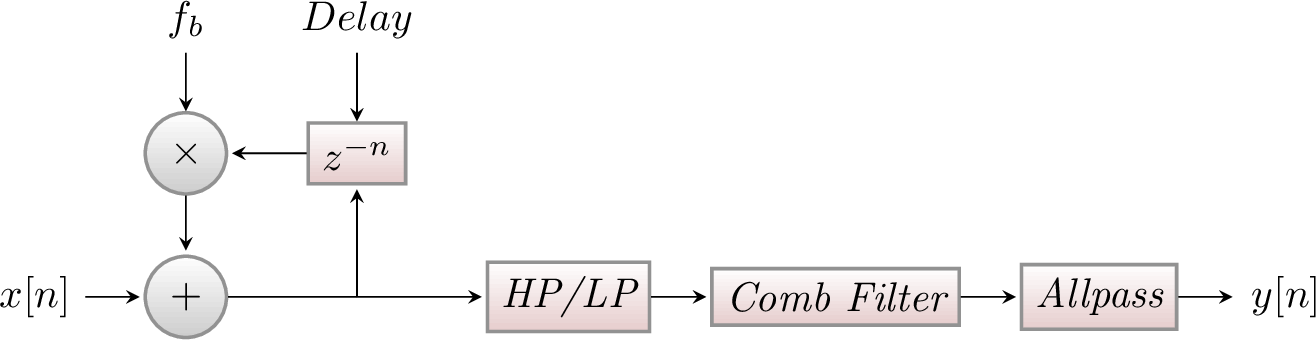
\includegraphics[scale=0.25]{zyn/effects/reverb.png}
   \caption{Reverb Circuit Diagram}
   \label{fig:reverb_circuit_diagram}
\end{figure}

\subsubsection{Effects / Reverb / User Interface}
\label{subsubsec:effects_edit_reverb_ui}

   The user-interface for the Reverb effect depends on whether it is used as a
   System effect or an Insertion effect.
   Observr \figureref{fig:effects_edit_reverb}, where
   the Insertion mode is shown.  In the System mode, only the light-blue
   portion of the user-interface appears.

\begin{figure}[H]
   \centering
%  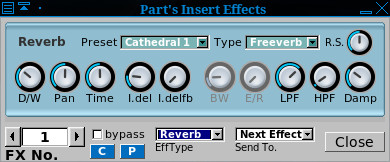
\includegraphics[scale=1.0]{bottom-panel/instrument-edit/Effects/effects-edit-reverb.jpg}
   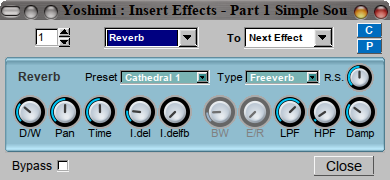
\includegraphics[scale=1.0]{1.3.9/effects-edit-reverb.png}
   \caption{Effects Edit, Reverb}
   \label{fig:effects_edit_reverb}
\end{figure}

   \begin{enumber}
      \item \textbf{Preset}
      \item \textbf{Type}
      \item \textbf{R.S.}
      \item \textbf{D/W}
      \item \textbf{Pan}
      \item \textbf{Time}
      \item \textbf{I.del}
      \item \textbf{I.delfb}
      \item \textbf{BW}
      \item \textbf{E/R}
      \item \textbf{LPF}
      \item \textbf{HPF}
      \item \textbf{Damp}
   \end{enumber}

  There is a fourth type we have screen captures for, but we can't seem
  to navigate to them now!  Are these now out-of-date screen captures?

   \begin{enumber}
      \item \textbf{FX No.}
      \item \textbf{bypass}
      \item \textbf{EffType}
      \item \textbf{Send To}
      \item \textbf{C}
      \item \textbf{P}
      \item \textbf{Close}
   \end{enumber}

   \setcounter{ItemCounter}{0}      % Reset the ItemCounter for this list.

   \itempar{Preset}{reverb!preset}
      Reverb Preset.

\begin{figure}[H]
   \centering
   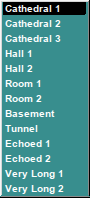
\includegraphics[scale=1.0]{bottom-panel/instrument-edit/Effects/reverb-preset-dropdown.png}
   \caption{Reverb Preset Dropdown}
   \label{fig:reverb_preset_dropdown}
\end{figure}

   Values: \texttt{Cathedral 1, Cathedral 2, Cathedral 3, Half 1, Half 2,
              Room 1, Room 2, Basement, Tunnel, Echoed 1, Echoed 2, Very Long
               1, Very Long 2}

   \itempar{Type}{reverb!type}
   Reverb Type.
   The combobox lets one select a reverb type.

\begin{figure}[H]
   \centering
   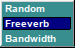
\includegraphics[scale=1.0]{bottom-panel/instrument-edit/Effects/reverb-type-dropdown.png}
   \caption{Reverb Type Dropdown}
   \label{fig:reverb_type_dropdown}
\end{figure}

   \begin{itemize}
      \item Freeverb is a preset. It was proposed by Jezar at Dreampoint.
      \item Bandwidth has the same parameters for the comb and allpass
         filters, but it applies a unison before the LPF/HPF. The unison’s
         bandwidth can be set using BW.
      \item Random chooses a random layout for comb and allpass each time the
         type or the roomsize is being changed.
   \end{itemize}

   Values: \texttt{Random, Freeverb, Bandwidth}

   \itempar{R.S}{reverb!room size}
   Reverb Room Size.
   The room size defines parameters only for the comb and allpass filters.

   \itempar{D/W}{reverb!dry/wet}
   Reverb Dry/Wet Setting.
   This setting controls much of the original signal is mixed with the
   reverb effect.

   \itempar{Pan}{reverb!pan}
   Reverb Panning.
   Pan lets one apply panning. This is the last process to happen.

   \itempar{Time}{reverb!time}
   Reverb Time.
   Set the duration of late reverb.
   Time controls how long the whole reverb shall take, including how slow
   the volume is decreased.

   \itempar{I.del}{reverb!initial delay}
   Reverb Initial Delay.
   The initial delay (I.del) is the time which the sounds need at least to
   return to the user.

   \itempar{I.delfb}{reverb!initial delay feedback}
   Reverb Initial Delay Feedback.
   Sets the initial delay feedback.
   The initial delay feedback (I.delfb) says how much
   of the delayed sound is added to the input.
   It is not recommended to use this setting together with
   low initial delays).

   \itempar{BW}{reverb!bandwidth}
   Reverb Bandwidth.

   \itempar{E/R}{reverb!e/r}
   Reverb E/R.
   Echo Reflection?  TODO!

   \itempar{LPF}{reverb!lpf}
   Reverb Lowpass Filter.
   This filter is applied before the comb filters.

   \itempar{HPF}{reverb!hpf}
   Reverb Highpass Filter.
   This filter is applied before the comb filters.

   \itempar{Damp}{reverb!damp}
   Reverb Damp.
   Damp determines how high frequencies are damped during the
   reverberation.  The dampening control (Damp) currently only allows to
   damp low frequencies. Its parameters are used by the comb and allpass
   filters.

   \itempar{FX No}{reverb!fx no.}
   Reverb FX Number.

   Values: \texttt{1 to 8?}

   \itempar{bypass}{reverb!fx bypass}
   Reverb FX Bypass.

   Values: \texttt{Off*, On}

   \itempar{EffType}{reverb!eff type}
   Reverb Effect Type.

   Values: \texttt{Reverb, EQ, Echo, etc. TODO}

   \itempar{Send To}{reverb!send to}
   Reverb Send To.
   This user-interface drop-down is shown only in the
   \textbf{Part / Edit / Effects} version of the effects panel.

   Values: \texttt{Next Effect, Part Out, Dry Out}

   \itempar{C}{reverb!copy}
   Reverb Copy.

   \itempar{P}{reverb!paste}
   Reverb Paste.

   \itempar{Close}{reverb!close}
   Close Window.

\subsubsection{Effects / Reverb / NRPN Values}
\label{subsubsec:effects_edit_reverb_nrpn}

   Effects can be controlled via "non-registered parameter numbers", or NRPNs.
   This section details the values supported by the Reverb effect.

   TODO:  detail the values supported by the Reverb effect.
   \index{todo!reverb nrpn values}

%-------------------------------------------------------------------------------
% vim: ts=3 sw=3 et ft=tex
%-------------------------------------------------------------------------------
